%% BioMed_Central_Tex_Template_v1.06
%%                                      %
%  bmc_article.tex            ver: 1.06 %
%                                       %

%%IMPORTANT: do not delete the first line of this template
%%It must be present to enable the BMC Submission system to
%%recognise this template!!

%%%%%%%%%%%%%%%%%%%%%%%%%%%%%%%%%%%%%%%%%
%%                                     %%
%%  LaTeX template for BioMed Central  %%
%%     journal article submissions     %%
%%                                     %%
%%          <8 June 2012>              %%
%%                                     %%
%%                                     %%
%%%%%%%%%%%%%%%%%%%%%%%%%%%%%%%%%%%%%%%%%


%%%%%%%%%%%%%%%%%%%%%%%%%%%%%%%%%%%%%%%%%%%%%%%%%%%%%%%%%%%%%%%%%%%%%
%%                                                                 %%
%% For instructions on how to fill out this Tex template           %%
%% document please refer to Readme.html and the instructions for   %%
%% authors page on the biomed central website                      %%
%% http://www.biomedcentral.com/info/authors/                      %%
%%                                                                 %%
%% Please do not use \input{...} to include other tex files.       %%
%% Submit your LaTeX manuscript as one .tex document.              %%
%%                                                                 %%
%% All additional figures and files should be attached             %%
%% separately and not embedded in the \TeX\ document itself.       %%
%%                                                                 %%
%% BioMed Central currently use the MikTex distribution of         %%
%% TeX for Windows) of TeX and LaTeX.  This is available from      %%
%% http://www.miktex.org                                           %%
%%                                                                 %%
%%%%%%%%%%%%%%%%%%%%%%%%%%%%%%%%%%%%%%%%%%%%%%%%%%%%%%%%%%%%%%%%%%%%%

%%% additional documentclass options:
%  [doublespacing]
%  [linenumbers]   - put the line numbers on margins

%%% loading packages, author definitions

% \documentclass[twocolumn]{bmcart}% uncomment this for twocolumn layout and comment line below
\documentclass{bmcart}

%%% Load packages
\usepackage[australian]{babel}
\usepackage[yyyymmdd]{datetime}
\renewcommand{\dateseparator}{--}
\usepackage{amsmath}
\usepackage{nccmath}
\usepackage{enumerate}
%\RequirePackage{natbib}
\RequirePackage{hyperref}
% \usepackage{helvet}
\usepackage{mathpazo}
\usepackage{courier}
\usepackage[style=ieee]{biblatex}
\bibliography{bib_ref.bib}
\usepackage[T1]{fontenc}
% \usepackage[utf8]{inputenc} %unicode support
%\usepackage[applemac]{inputenc} %applemac support if unicode package fails
%\usepackage[latin1]{inputenc} %UNIX support if unicode package fails
\usepackage{graphicx}

%%%%%%%%%%%%%%%%%%%%%%%%%%%%%%%%%%%%%%%%%%%%%%%%%
%%                                             %%
%%  If you wish to display your graphics for   %%
%%  your own use using includegraphic or       %%
%%  includegraphics, then comment out the      %%
%%  following two lines of code.               %%
%%  NB: These line *must* be included when     %%
%%  submitting to BMC.                         %%
%%  All figure files must be submitted as      %%
%%  separate graphics through the BMC          %%
%%  submission process, not included in the    %%
%%  submitted article.                         %%
%%                                             %%
%%%%%%%%%%%%%%%%%%%%%%%%%%%%%%%%%%%%%%%%%%%%%%%%%


%%% Put your definitions there:
\startlocaldefs
\endlocaldefs
\usepackage{geometry}
\geometry{letterpaper,margin=2.5cm}

%%% Begin ...
\begin{document}

%%% Start of article front matter
\begin{frontmatter}

% \begin{fmbox}
\dochead{01 June 2018 | Bioengineering 420 Medical Imaging | M. O'Donnell}

%%%%%%%%%%%%%%%%%%%%%%%%%%%%%%%%%%%%%%%%%%%%%%
%%                                          %%
%% Enter the title of your article here     %%
%%                                          %%
%%%%%%%%%%%%%%%%%%%%%%%%%%%%%%%%%%%%%%%%%%%%%%

\title{A Review of Computer-Aided CT and MRI in Literature and the Clinic}

%%%%%%%%%%%%%%%%%%%%%%%%%%%%%%%%%%%%%%%%%%%%%%
%%                                          %%
%% Enter the authors here                   %%
%%                                          %%
%% Specify information, if available,       %%
%% in the form:                             %%
%%   <key>={<id1>,<id2>}                    %%
%%   <key>=                                 %%
%% Comment or delete the keys which are     %%
%% not used. Repeat \author command as much %%
%% as required.                             %%
%%                                          %%
%%%%%%%%%%%%%%%%%%%%%%%%%%%%%%%%%%%%%%%%%%%%%%

\author{\textit{Aidan Johnson, Department of Electrical Engineering, University of Washington}}

%%%%%%%%%%%%%%%%%%%%%%%%%%%%%%%%%%%%%%%%%%%%%%
%%                                          %%
%% Enter the authors' addresses here        %%
%%                                          %%
%% Repeat \address commands as much as      %%
%% required.                                %%
%%                                          %%
%%%%%%%%%%%%%%%%%%%%%%%%%%%%%%%%%%%%%%%%%%%%%%


%%%%%%%%%%%%%%%%%%%%%%%%%%%%%%%%%%%%%%%%%%%%%%
%%                                          %%
%% Enter short notes here                   %%
%%                                          %%
%% Short notes will be after addresses      %%
%% on first page.                           %%
%%                                          %%
%%%%%%%%%%%%%%%%%%%%%%%%%%%%%%%%%%%%%%%%%%%%%%

% \begin{artnotes}

% \end{artnotes}

% \end{fmbox}% comment this for two column layout

%%%%%%%%%%%%%%%%%%%%%%%%%%%%%%%%%%%%%%%%%%%%%%
%%                                          %%
%% The Abstract begins here                 %%
%%                                          %%
%% Please refer to the Instructions for     %%
%% authors on http://www.biomedcentral.com  %%
%% and include the section headings         %%
%% accordingly for your article type.       %%
%%                                          %%
%%%%%%%%%%%%%%%%%%%%%%%%%%%%%%%%%%%%%%%%%%%%%%


\begin{abstract} % abstract
Developing clinically integrated computer-aided diagnosis (CAD)---the 3D reconstruction and the computational analysis of the images produced from the complementary modality pair, computed tomography (CT) and magnetic resonance (MR) imaging---pose challenging computer vision and machine learning problems. Despite the challenges, advances in CAD techniques permit it to provide more complete and valuable patient information that aides clinicians in the detection, diagnosis, and treatment of disease. Currently, CAD has started to be translated in the clinic, thanks to improvements of the software algorithms and hardware processing power. This paper focuses on present and future CAD clinical translations. Literature will be surveyed in order to discuss the clinical applicability and benefits of these computational methods.
\end{abstract}

%%%%%%%%%%%%%%%%%%%%%%%%%%%%%%%%%%%%%%%%%%%%%%
%%                                          %%
%% The keywords begin here                  %%
%%                                          %%
%% Put each keyword in separate \kwd{}.     %%
%%                                          %%
%%%%%%%%%%%%%%%%%%%%%%%%%%%%%%%%%%%%%%%%%%%%%%

% \begin{keyword}

%\end{keyword}


% \end{fmbox}% uncomment this for twcolumn layout

\end{frontmatter}

%%%%%%%%%%%%%%%%%%%%%%%%%%%%%%%%%%%%%%%%%%%%%%
%%                                          %%
%% The Main Body begins here                %%
%%                                          %%
%% Please refer to the instructions for     %%
%% authors on:                              %%
%% http://www.biomedcentral.com/info/authors%%
%% and include the section headings         %%
%% accordingly for your article type.       %%
%%                                          %%
%% See the Results and Discussion section   %%
%% for details on how to create sub-sections%%
%%                                          %%
%% use \cite{...} to cite references        %%
%%  \cite{koon} and                         %%
%%  \cite{oreg,khar,zvai,xjon,schn,pond}    %%
%%  \nocite{smith,marg,hunn,advi,koha,mouse}%%
%%                                          %%
%%%%%%%%%%%%%%%%%%%%%%%%%%%%%%%%%%%%%%%%%%%%%%

%%%%%%%%%%%%%%%%%%%%%%%%% start of article main body
% <put your article body there>
\section*{Introduction}
For more than 80 years, plain film X-ray radiography dominated as medical imaging modality in the clinic. The \textit{status quo} changed in the 1970s when the first X-ray computed tomography (CT) scanner was introduced. By the 1990s, after a series of technological improvements, CT developed into a fast-scanning and a high spatial resolution imaging modality. CT images, now a clinical staple, are reconstructed from scanned slices of the human body, using the different X-ray absorption properties of anatomical tissues and structures. CT has a broad set of medical applications besides radiology \cite{rubin_computed_2014}. It is commonly used in neurology, hepatology, pulmonology, cardiology, and oncology. However, unlike magnetic resonance imaging (MRI), CT suffers from the disadvantages of harmful ionising radiation exposure and poor soft tissue contrast (e.g., white and grey matter in the brain) \cite{ward_mri:_2015}, \cite{radue_introduction_2016}. For these reasons, and the flexibility of reconstruction, MRI gained dominance especially in cognitive and neural sciences.
\par Rather than diving into the proverbial deep end and providing a primer of the fundamentals of medical imaging modalities of CT and magnetic resonance (MR), this paper will only give a relatively brief and abstract review. (Plenty of references found elsewhere in books and journals provide a far more rigorous treatment of CT and MRI.) Since CT and MRI are non-direct imaging systems, there is not a one-to-one mapping of the image subject to pixel space in terms of data acquisition as there is in ultrasound, for example. Instead, the image data voxels (3D pixels) must be measured multiple times to reconstruct the discrete image matrix of pixels \cite{adam_grainger_2015}. In CT, a single X-ray projection maps to one angular line of the Fourier domain, and in MRI, a single MR scan maps to one line of the Fourier domain (\textit{k}-space) \cite{farncombe_medical_2014}, \cite{plewes_physics_2014}. Nevertheless, they are similar imaging modalities in how they image or `slice' a specimen (as in the Greek root, \textit{tomos}, for `cut') \cite{liang_principles_2000}. The primary focus of this paper will be the current clinical and yet-to-be translated computer-aided diagnosis and therapy tools that pose potential benefits in the clinical setting. 
\par CAD---the 3D reconstruction and the computational analysis of the images produced from the complementary modality pair, CT and MR imaging---provides more complete patient information, thus aiding the limited-supply of clinicians in the detection, diagnosis, and treatment of disease \cite{van_ginneken_computer-aided_2011}. Despite the potential advances of integrating CAD into medical diagnostics and therapies, developing these techniques for CT and MR imaging pose challenging computer vision and machine learning problems. Nonetheless, CAD has begun clinical translation, which will continue as the computational speed and algorithmic accuracy and precision improve, in addition to a reduction in the required human interaction (quality assurance). The methods for segmentation---the division of the image into anatomical or structural regions of interest to augment readability and interpretability for clinicians---will be surveyed from technical literature and will be discussed for beneficial clinical applicability \cite{van_ginneken_computer-aided_2011}.

\section*{Background}
The main topic of clinical application in CAD research has been detection. This entails improving the canonical steps of CAD. These steps, with general definitions, are \cite{van_ginneken_computer-aided_2011}:
\begin{enumerate}[\indent \arabic{enumi}.]
    \item preprocessing: removal of noise in image.
    \item segmentation: division of image into anatomic regions using computer vision algorithms.
    \item candidate detection: flagging of regions requiring human attention.
    \item feature extraction: vectorisation of the candidates and their features.
    \item classification: determination of whether a region is normal or abnormal using supervised machine learning (where labelled training data is required) algorithms.
    \item output: reporting of the suspicious candidate results.
\end{enumerate}
In the next sections, some of these steps will be explained and explored in greater detail. (Classification, which is an expansive topic in its own right, due to the development of machine learning algorithms such as \textit{k}-means clustering, \textit{k}-nearest-neighbour classification, support vector machines, and neural networks to name a few, will not be discussed \cite{pham_current_2000}, \cite{van_ginneken_computer-aided_2011}, \cite{sharma_automated_2010}.) Reconstruction, as well as segmentation and feature (edge and region) detection, approaches will be analysed in the upcoming sections in addition to a higher level discussion of other CAD methods. Since CT and MR are both tomographic modalities, most of the image processing approaches discussed are cross-applicable. Their ultimate difference is image contrast. 
\par The motivation for detection is to improve the diagnostic process, and therefore the quality of care, in clinic. With CT, radiologists are in limited supply, whilst the cost and the demand for radiology imaging has increased. Moreover, CT and MRI have augmented clinicians' understanding of anatomy, physiology, and pathology, and has improved disease detection, characterisation, and management. To improve diagnosis, the promises of CAD satisfy the goals of bettering the lesion detection accuracy, the expediency, and the quantitative evaluation of the diagnostic process. A few specific lesion detection applications of CAD are in: mammography and breast cancer screening for mass lesions and microcalcification clusters; colonography and polyp detection; and pulmongraphy and malignant lung nodule detection. Beyond these diagnosis motivations, to be beneficial in the clinical setting, a CAD system needs to offset the costs of itself whether by saving time or improving clinician performance, integrate into the clinical workflow without interruption, and not add liability \cite{van_ginneken_computer-aided_2011}. In addition to augmenting the clinician in diagnosis, CAD can guide the planning and monitoring therapy, surgery, and treatments \cite{hutton_software_2003}, \cite{banik_landmarking_2009}, \cite{pham_current_2000}, \cite{sharma_automated_2010}. Exclusively with CT, although a major imaging modality, the harmful effects of ionising radiation exposure are also a major clinical concern. The link between X-ray radiation exposure during CT imaging and the elevated risk of cancer is well known. The risk is especially acute in paediatric patients \cite{liu_model-based_2014}.

\section*{Image Reconstruction}
CT reconstruction methods can be divided into two types. They differ in how the (X-ray or magnetic) attenuation value for each voxel is assigned. The first method type is analytical. This method assumes projections are measured continuously and approximates using interpolation to account for the cone-beam 3D geometry of the CT imaging system. As the alternative to the analytical filtered back projection (FBP) reconstruction, iterative reconstruction (IR) either statistically models the image noise inherently present or models the system geometry \cite{geyer_state_2015}, \cite{beister_iterative_2012}. Both of these approaches are examined below.

\subsection*{Analytical Reconstruction}
Both CT and MRI rely on beautiful mathematics. Perhaps one of the most elegant theorems of medical imaging, the Central Slice Theorem, also known as the Fourier-Slice Theorem or Projection-Slice Theorem, states that a slice of the 2D Fourier Transform of the imaged object is equal to the 1D Fourier Transform a projection of that object \cite{gonzalez_digital_2008}. This fundamental theorem allows for a CT scan to be reconstructed image. Mathematically, for an object $f(x,y)$ and its Fourier Transform (FT) $F(u,v)$ where $u=\omega\cos\theta$ and $v=\omega\sin\theta$ (polar coordinates), the theorem can be written as:
\begin{ceqn}
\begin{align}
        F(\omega\cos\theta,\omega\sin\theta)=\int_{-\infty}^{\infty} \int_{-\infty}^{\infty} f(x,y)\exp{(-2\pi j (x\omega\cos{\theta}+y\omega\sin{\theta}))} \mathrm{d}x \mathrm{d}y
\end{align}
\end{ceqn}
\begin{ceqn}
\begin{align}
        F_{polar}(\theta,\omega)=\int_{-\infty}^{\infty} p(\theta,t)\exp{(-2\pi j t \omega)}\mathrm{d}t
\end{align}
\end{ceqn}
where the projection of $f(x,y)$ is the line integral through the object or the Radon Transform of the object. That is
\begin{ceqn}
\begin{align}
        p(\theta,t)=\int\limits_{L(\theta,t)}f(x,y) \mathrm{d}s = \int_{-\infty}^{\infty} \int_{-\infty}^{\infty} f(x,y)\delta{(x\cos{\theta}+y\sin{\theta}-t)} \mathrm{d}x \mathrm{d}y
\end{align}
\end{ceqn}
\par The image can reconstructed by simply taking the inverse 2D FT of the 1D FT of one projection to get one slice. Unfortunately for CT, this reconstruction method is inefficient. It is although used by MRI \cite{farncombe_medical_2014}. Instead the parallel-beam filtered backprojection is the standard reconstruction method for CT. There are two steps in FBP. First, a ramp filter (often a Shepp-Logan filter) kernel $h_R$ is convolved with the parallel-beam projections $p$ in the radial direction $t$. Then, the filtered projection $p_F$ is backprojected to the image space for angles $theta$ between $0 \deg$ and $180 \deg$. After substituting the Central Slice Theorem, the mathematics simplifies to:
\begin{ceqn}
\begin{align}
        f(x,y)=\int_{0}^{\pi} \int_{-\infty}^{\infty} p(\theta,t)h_R(t-t') \mathrm{d}t' \mathrm{d}\theta
\end{align}
\end{ceqn}
The image produced from FBP has wide clinical acceptance. Nonetheless, there are limitations to FBP. Namely, not considering the 3D cone-beam geometry introduces errors. It also makes approximation and interpolation assumptions. While the image reconstructed is subjectively sharper in comparison to the iterative method, increased noise is introduced in FBP \cite{geyer_state_2015}. 

\subsection*{Iterative Reconstruction}
In contrast, an iterative approach has certain advantages. By modelling the 3D system geometry, IR has been found to be reduce patient radiation exposure or dosage in a range of \textasciitilde{}30\%--60\% as well as reduce noise by \textasciitilde{}50\% \cite{patino_iterative_2015}, \cite{beister_iterative_2012}. Before delving in further, it would be apt to briefly foray into the state-of-the-art for computing hardware.

\subsubsection*{IR \& Graphics Processing Units}
IR algorithms reduce dosage because it more precisely models the projection data acquisition process \cite{liu_model-based_2014}, \cite{beister_iterative_2012}. IR had not been widely implemented because of its heavy computational cost \cite{geyer_state_2015}, \cite{liu_model-based_2014}. Advances in hardware have enabled IR, which was first proposed in the 1970s with the introduction of CT, to be reconsidered as a viable reconstruction algorithm \cite{liu_model-based_2014}, \cite{geyer_state_2015}. Improvements in semiconductor and transistor technology, as predicted by Moore's law, have increased the computational speed of processors.
\par In IR, forward- and back-projections are computed in parallel. Due to the parallel nature of the computations performed in IR, the serial process threading of central processing units (CPUs) made IR inefficient \cite{beister_iterative_2012}. Then entered graphics processing units (GPUs), which were designed for the parallel processing needs of computer graphics. GPUs in comparison are more energy efficient and cost-effective than distributed CPUs. The GPU architecture is such that one has parallel functional units in individual cores. While CPUs have a separate control unit per core (\textasciitilde{}4--12 total cores), GPUs have the same instruction set (kernel) and control unit for its thread processors. Many thousands of thread (an instance of a kernel) processors comprise a one of a GPU's \textasciitilde{}20--40 cores. GPUs, because of this architecture are readily implemented for the parallel computation requirements of iterative methods. GPUs continue to increase in thread processors, clock speed, and on-board memory \cite{smistad_medical_2015}. 

\subsubsection*{IR Approaches}
 In general, for IR, an estimated raw object data is compared to measured raw object data. The difference in these datasets is then used to change the data estimation. This continues until the difference between the actual and artificial data is less than a predefined threshold \cite{liu_model-based_2014}. The general flow for the IR algorithm are best summarised visually, as is provided below in Figure \ref{fig:ir_flow}.
\begin{figure}[h!] 
  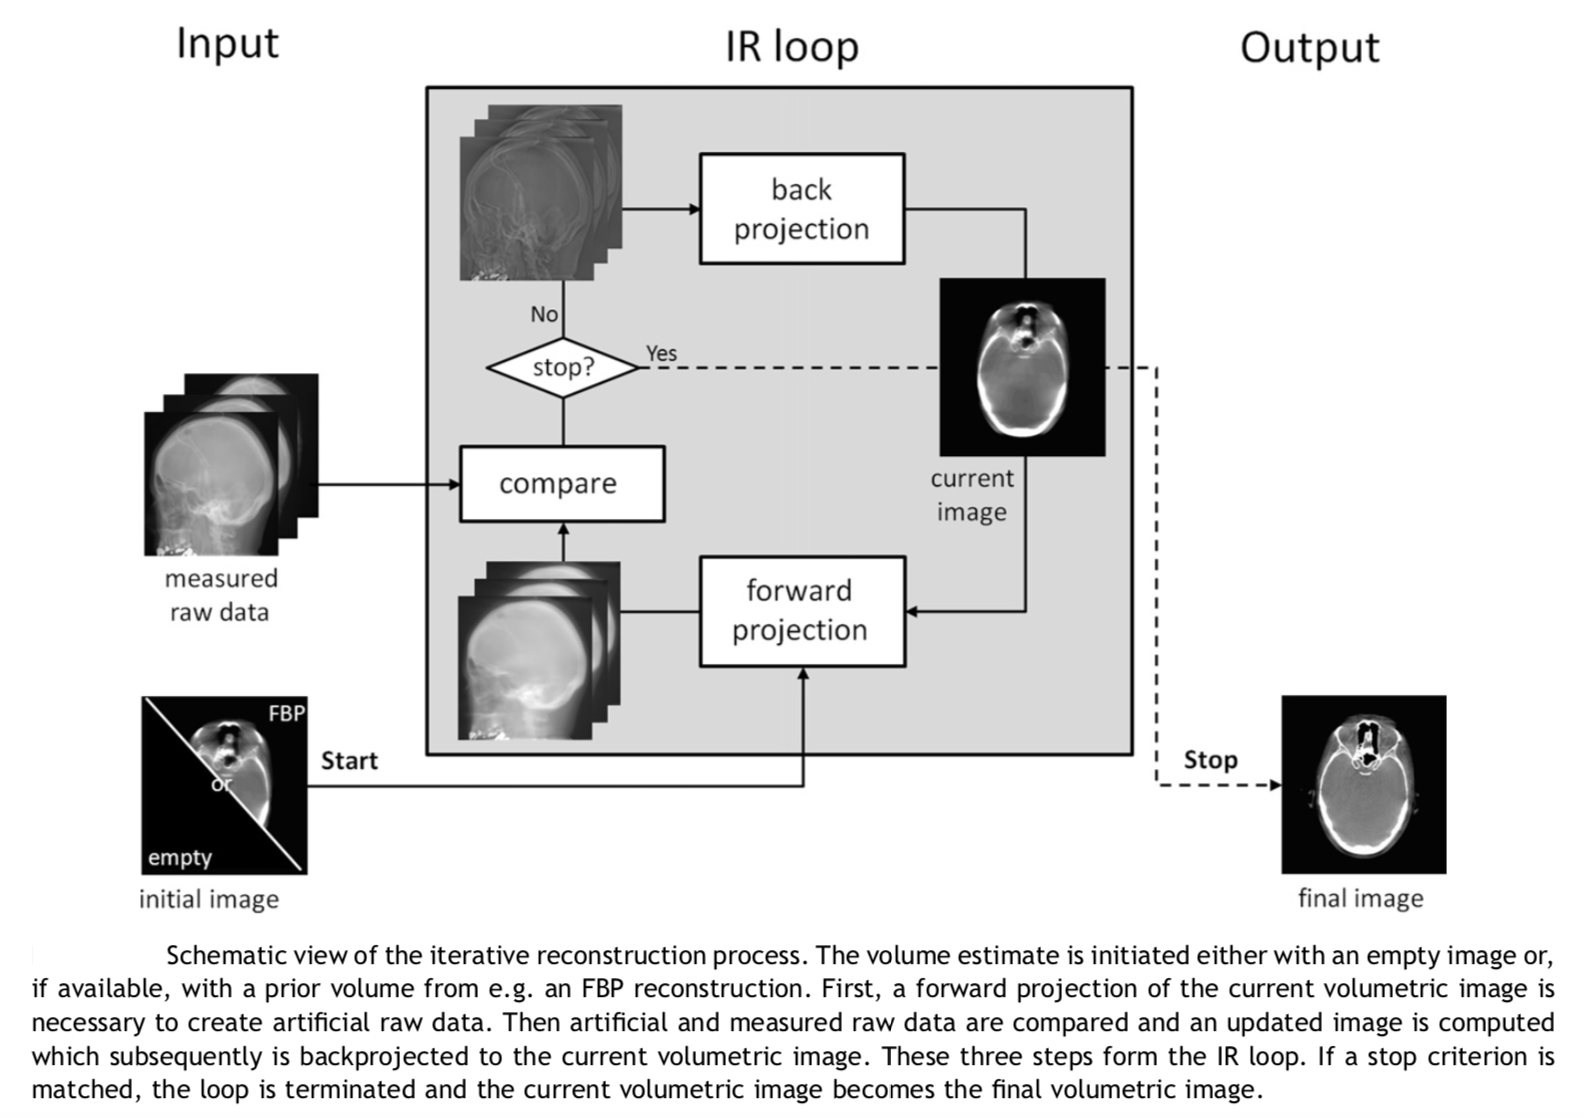
\includegraphics[scale=.5]{figures/beister_ir.png}
  \caption{\csentence{\cite{beister_iterative_2012}} IR algorithmic flow.}
  \label{fig:ir_flow}
\end{figure}
\par Within the iterative approaches to reconstructions, there two different methods of modelling. One paradigm is a model-based IR (MBIR). An objective or cost function is minimised for the actual system, statistical noise, and the \textit{a priori} data model. The system is modelled geometrically, and usually model the X-rays as going through voxels instead of a point to an area of pixels on a detector. Each pixel is a separate thread on a GPU \cite{beister_iterative_2012}. The other paradigm is adaptive statistical IR (ASIR). Noise in either paradigm is attributed to the random fluctuations of the X-ray photons, however in ASIR, the system is not modelled. Thus, ASIR is considered to be inferior to MBIR \cite{liu_model-based_2014}. For sake of comparison, Figure \ref{fig:ir_table} summarises the notable advantages and disadvantages of IR techniques.
\begin{figure}[h!] 
  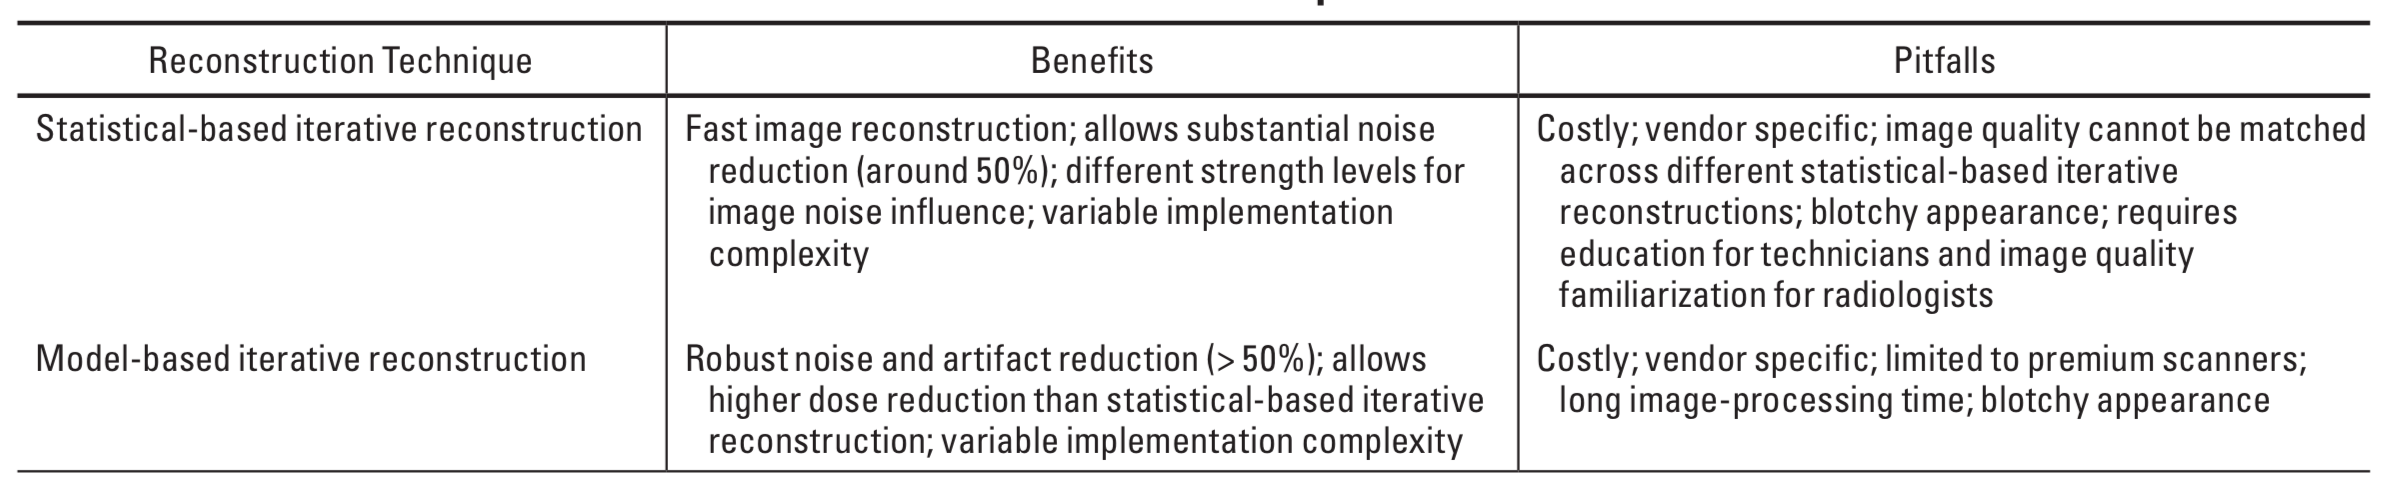
\includegraphics[scale=.39]{figures/patino_ir.png}
  \caption{\csentence{\cite{patino_iterative_2015}} Comparison of cost-benefits of the two IR types.}
  \label{fig:ir_table}
\end{figure}
The count of the photons that pass from the X-ray collimator, through the patient, to the detector are modelled as having a Poisson distribution. Instead of an objective function, data fitting algorithms such as maximum likelihood in conjunction with expectation maximisation, least squares, and ordered subset convex (OSC). Least squares is difficult to parallelise while OSC is easily parallelise on GPUs \cite{beister_iterative_2012}. Additionally, IR algorithms, which are used to reduce dosage as discussed earlier, have been implemented commercially by the leading manufacturers (e.g., GE, Philips, Siemens, and Toshiba). Since their methods are proprietary (black-boxes), little detail is known. Some of their algorithms are hybrids of the two paradigms, and even with FBP \cite{geyer_state_2015}.
\par Special attention will be paid here to OSC, as it translates well to the GPU architecture and illustrates the IR process well. Initially, a subset of the X-ray projections are collected for estimating the image. After each iteration of the estimation, a new subset is selected such that the angular distance separating the new subset and the previously used subset is maximised. If $N_p$ is the total number of projections, the selected subsets for the $k$th iteration out of $K$ is $s_k$. The next estimate update calculated using the equation:
\begin{ceqn}
\begin{align}
    f_{v+1}=f_v+f_v{\frac{R_{v}^{T}(\exp{(-R_v f_v)}-\exp{(-p)})}{R_{v}^{T}(\exp{(-R_v f_v)}R_v f_v)}}
\end{align}
\end{ceqn}
where $R_v$ is the Radon Transform (forward-projection) for the $v$th subset in iteration $k$, where $R_{v}^{T}$ is the back-projection, and $\exp{-p}$ is the measured intensities. From this equation we can see how parallel processing relieves the computational burden.

\section*{Segmentation}
An unsolved challenge in medical imaging, segmentation is a essential task in computer vision. In my many-hours literature search, I came across a quote that seemed to capture the \textit{raison d'\^{e}tre} of medical image segmentation. `According to Euclid, the whole is defined by the sum of the parts. In image segmentation, we attempt to find the parts' \cite{acton_biomedical_2009}. And in this section, I intend to illuminate just that. 
\par Segmentation can be formally defined as partitioning the image into non-intersection and contiguous regions $S_k$ (segments or subsets) that in union form the entire image domain $\Omega$. Or in set theory notation, for $S_k \subset \Omega$ and $K$ segmentation classes:
\begin{ceqn}
\begin{align}
    \Omega = \bigcup_{k=1}^{K} S_k, \mathrm{\quad where \quad} S_k \cap S_j = \emptyset
\end{align}
\end{ceqn}
Formal definitions aside, there are many modes of segmentation, each with their merits. The four types of segmentation boil down to: (1) edge-based; (2) region-based; (3) deformable model-based; and (4) knowledge-based.

\subsection*{Edge-Based}
The most basic segmentation method is pixel Hounsfield Units (attenuation in HU) histogram thresholding. After a threshold is estimated, Otsu's method can be applied to partition the histogram to maximise the inter-class difference \cite{rafati_comparison_2014}. Excluding thresholding, the general principle of edge detection centres around the gradient of the image. From introductory calculus we know for a 2D function $f(x,y)$ (like an image), the gradient is the sum of the partial derivatives of the function as vectors. Fortunately for us, the medical images we work with are discrete. For discrete functions the derivative is simply the finite difference. So the gradient can be expressed in terms of the horizontal ($G_x$) and vertical ($G_y$) gradient \cite{banik_landmarking_2009}.
\begin{ceqn}
\begin{align}
    \nabla f(x,y) \approx |G_x(x,y)|+|G_y(x,y)|=|f(x,y)-f(x-1,y)|+|f(x,y)-f(x,y-1)| 
\end{align}
\end{ceqn}
Instead of calculating the gradient using this equation, we can correlate kernel operators to get the gradient. Popular $3\times3$ kernels are the Sobel and Prewitt operators, and the $2\times2$ Roberts operators. The horizontal and vertical gradients kernels, gradient magnitude, and angle for each are as follows \cite{rafati_comparison_2014}.
\begin{ceqn}
\begin{align}
  S_x = \begin{bmatrix}
        -1 & 0 & 1  \\
        -2 & 0 & 2 \\
        -1 & 0 & 1
      \end{bmatrix}
      \quad
  S_y = \begin{bmatrix}
        -1 & -2 & -1  \\
         \phantom{-}0 &  \phantom{-}0 &  \phantom{-}0 \\
         \phantom{-}1 &  \phantom{-}2 &  \phantom{-}1
      \end{bmatrix}
      \quad
  |S|=\sqrt{{S_x}^2+{S_y}^2}
  \quad
  \theta=\arctan{(S_y/S_x)}
\end{align}
\end{ceqn}
\begin{ceqn}
\begin{align}
  P_x = \begin{bmatrix}
         \phantom{-}1 & \phantom{-}1 & \phantom{-}1  \\
         \phantom{-}0 & \phantom{-}0 & \phantom{-}0 \\
        -1 & -1 & -1
      \end{bmatrix}
      \quad
  P_y = \begin{bmatrix}
        -1 & 0 & 1  \\
        -1 & 0 & 1 \\
        -1 & 0 & 1
      \end{bmatrix}
            \quad
  |P|=\sqrt{{P_x}^2+{P_y}^2}
  \quad
  \theta=\arctan{(P_y/P_x)}
\end{align}
\end{ceqn}
\begin{ceqn}
\begin{align}
  R_x = \begin{bmatrix}
        1 & \phantom{-}0  \\
        0 & -1
      \end{bmatrix}
      \quad
  R_y = \begin{bmatrix}
        \phantom{-}0 & 1 \\
        -1 & 0
      \end{bmatrix}
      \quad
  |R|=\sqrt{{R_x}^2+{R_y}^2}
  \quad
  \theta=\arctan{(R_y/R_x)}-3\pi/4
\end{align}
\end{ceqn}
Alternatively, the omni-directional edge-detector Laplacian of pixel intensity $I(x,y)$ is 
\begin{ceqn}
\begin{align}
    L(x,y)={\partial^2 I}/{\partial x^2} + {\partial^2 I}/{\partial y^2}
\end{align}
\end{ceqn}
or as equivalent kernels:
\begin{ceqn}
\begin{align}
  L = \begin{bmatrix}
         \phantom{-}0 & \phantom{-}1 & \phantom{-}0  \\
         \phantom{-}1 & -4 & \phantom{-}1 \\
         \phantom{-}0 & \phantom{-}1 & \phantom{-}0 
      \end{bmatrix}
      \quad
      \mathrm{or}
      \quad
   \begin{bmatrix}
         \phantom{-}1 & \phantom{-}1 & \phantom{-}1  \\
         \phantom{-}1 & -8 & \phantom{-}1 \\
         \phantom{-}1 & \phantom{-}1 & \phantom{-}1
    \end{bmatrix}
      \quad
      \mathrm{or}
      \quad
   \begin{bmatrix}
         -1 & \phantom{-}2 & -1  \\
         \phantom{-}2 & -4 & \phantom{-}2 \\
         -1 & \phantom{-}2 & -1 
    \end{bmatrix}
\end{align}
\end{ceqn}
\par All of these gradient operators can detect edges. After the gradient operation, the strength of the edge inferred from the gradient magnitude. Edges with a strength greater than a threshold are kept while the other fake and weak edges are removed \cite{sharma_automated_2010}. The Hough Transform, which maps line to points and vice-versa. In the Hough space $\rho$-$\theta$ plane, intersections of lines  (i.e., points) correspond to lines in Cartesian space $x$-$y$ plane. The equation $\rho=x\cos\theta + y\sin\theta$ transforms Cartesian lines given by $y=mx+b$ to the Hough plane \cite{banik_landmarking_2009}. The last edge detecting operation to be highlighted is the Canny edge detector; its algorithm is \cite{rafati_comparison_2014}:
\begin{enumerate}[\indent \arabic{enumi}.]
    \item Smooth image using filtering techniques;
    \item Find high spatial derivatives from the image gradient;
    \item Attenuate pixels not at the maximum gradient;
    \item Perform hysteresis by applying a high/low threshold where pixels with an intensity:
    \begin{enumerate}
        \item above the high threshold are determined as part of an edge.
        \item in between the high and low threshold are determined to be a weak edge.
        \item below the low threshold are attenuated to zero.
    \end{enumerate}
\end{enumerate}
\subsection*{Region-Based}
Regions can be thought of as segmented partitions. At a most basic level, after a distance metric has been selected and from initial `seeds', pixels that are similar according to the metric are merged into a region. The similarity metric could be whether the pixel intensity value is within a certain range corresponding to greyscale, texture, or colour \cite{banik_landmarking_2009}. Conversely, the entire image could be split into regions based on whether pixels are dissimilar. Lastly, an image could be divided into equal square quadrants. Then recursively subdivide a square if it is determined not to be homogeneous according to some metric. Merge the recursed subdivided quadrants if they together would be homogeneous. This process would continue until no further merges or splits can occur, or when a stopping iteration parameter is reached \cite{sharma_automated_2010}. The utility of region segmentation is it allows clinicians to divide a medical image into anatomic regions which augments differentiation of anatomical structures \cite{van_ginneken_computer-aided_2011}, \cite{oliveira_medical_2014}.

\subsection*{Deformable Model-Based}
The approaches in this class are more mathematically complex. The common theme between the registration approaches is that they all optimise a cost or objective function to find an optimal boundary curve or active contour. A snake, or the contour curve, traverses the gradient surface $f(x,y)=|\nabla I|^2=({\partial I}/{\partial x})^2+({\partial I}/{\partial y^2})^2$ of the image $I(x,y)$. In short, the snake is initialised near the boundary of the region of interest of the object image. The snake then evolves to the boundary as governed by the minimisation of the cost function. 
\par This specific function, called the energy function, governs the snake's evolution, or contour tracking, and its stiffness or elasticity. The energy function is defined as $E_{total}=E_{internal}+E_{external}$, in terms of the curve position $(x,y)$. The snake is parametrically defined by $s$ as $(x,y)=(X(s),Y(s))$. The internal and external energy functions are defined as:
\begin{ceqn}
\begin{align}
    E_{external}(X,Y) = - \int_0^1 f(X,Y)\mathrm{d}s
\end{align}
\end{ceqn}
\begin{ceqn}
\begin{align}
    E_{internal}(X,Y)=\frac{1}{2} \int_0^1 \alpha (|\frac{\mathrm{d}X}{\mathrm{d}s}|^2 + |\frac{\mathrm{d}Y}{\mathrm{d}s}|^2) + \beta (|\frac{\mathrm{d}^2X}{\mathrm{d}s^2}|^2 + |\frac{\mathrm{d}^2Y}{\mathrm{d}s^2}|^2)
\end{align}
\end{ceqn}
where $\alpha$ and $\beta$ are tuning parameters. Gradient descent will allow us to at least find a local minimum and at best a global minimum. The minimisation of the energy function $E_{total}$ can be accomplished in a few ways; namely, with the Lagrangian, dynamic programming, and other greedy algorithms \cite{el-baz_biomedical_2017}. All three of these algorithmic approaches are computation-heavy, so we see that solving for the active contour methods is highly suitable for GPU implementation \cite{smistad_medical_2015}. Contouring of a region of interest can also be performed manually using a pointer peripheral. This method uses morphological operations---erosion and dilation---to combine desired regions \cite{brock_image_2014}.

\subsection*{Knowledge-Based}
Atlas-based segmentation requires building a database that compiles expert knowledge of anatomy, physiology, pathology, and the shape, size, texture, and relative position of organs and soft tissues (an atlas) \cite{banik_landmarking_2009}, \cite{sharma_automated_2010}. The captured images are then cross-referenced to the atlas for the purpose of registration and localisation of organs and anatomical structures \cite{banik_landmarking_2009}. Already commercial atlases implemented in clinical-use software have been made available. Currently, commercial software has accurately segmented head-and-neck and brain anatomy \cite{brock_image_2014}. To help achieve necessary reliability, landmarks are necessary for aligning the clinical image with the database reference image. A suitable landmark for image alignment has: (1) stable locations; (2) non-variable characteristics as result of abnormalities; and (3) easy to detect characteristic features. Examples that satisfy these requirements include the spine, spinal canal, rib structure, diaphragm, pelvis, thoracic cage, kidneys, liver, and spleen \cite{banik_landmarking_2009}.
\par The `sensed' image is aligned with the reference image to establish a one-to-one mapping or correspondence \cite{pham_current_2000}. Essential for aligning images taken at different angles and distances are affine transforms. With translation $t$, rotation $\theta$, and scaling $s$ for an 2D (on the $x$-$y$ plane) image $\vec{a}$ transformed to image $\vec{b}$ using a transformation matrix so that: \cite{zitova_image_2003}:
\begin{ceqn}
\begin{align}
    \begin{bmatrix}
    \vec{b_x} \\
    \vec{b_y} \\
    1
    \end{bmatrix}
    = \begin{bmatrix}
         s_x \cos \theta & s_x \sin \theta & t_x  \\
         -s_y \sin \theta & s_y \cos \theta & t_y \\
         0 & 0 & 1 
    \end{bmatrix}
    \begin{bmatrix}
    \vec{a_x} \\
    \vec{a_y} \\
    1
    \end{bmatrix}
\end{align}
\end{ceqn}
The affine transform stretches and skews the image as desired \cite{hajnal_medical_2001}. The affine transform can also be expanded high dimensions (e.g., 3D) \cite{brock_image_2014}. A more general algorithm for aligning images is the scale invariant feature transform (SIFT). This algorithm first determines descriptors and aligns them between images \cite{el-baz_biomedical_2017}.
\par The final atlas-based segmentation method to be explored is the mutual information metric. The theory behind mutual information (MI) has its origins in Claude Shannon's Information Theory. MI enables the features, both anatomical and functional, in the reference to be compared with the image of the patient \cite{zitova_image_2003}. MI has proven to be a highly robust metric. Entropy, which can be defined the information contained in the image or as the uncertainty of the image's pixel values. Shannon's definition of entropy, for the probability of finding a pixel with intensity $p_i$,  is \cite{hutton_software_2003}: 
\begin{ceqn}
\begin{align}
	H = - \sum_i p_i \log{p_i}
\end{align}
\end{ceqn}
The mutual information between two images $a$ and $b$ is then:
\begin{ceqn}
\begin{align}
	MI(a,b) = H(a)+H(b)-H(a,b)
\end{align}
\end{ceqn}
for a joint entropy $H(a,b)$ using the joint probability distribution function for those images \cite{hajnal_medical_2001}. A particular alignment can be optimised by maximising the MI between the reference and sensed image \cite{hutton_software_2003}. Figure \ref{fig:hutton_mi} below visually summarises the principle. 
\begin{figure}[h!] 
  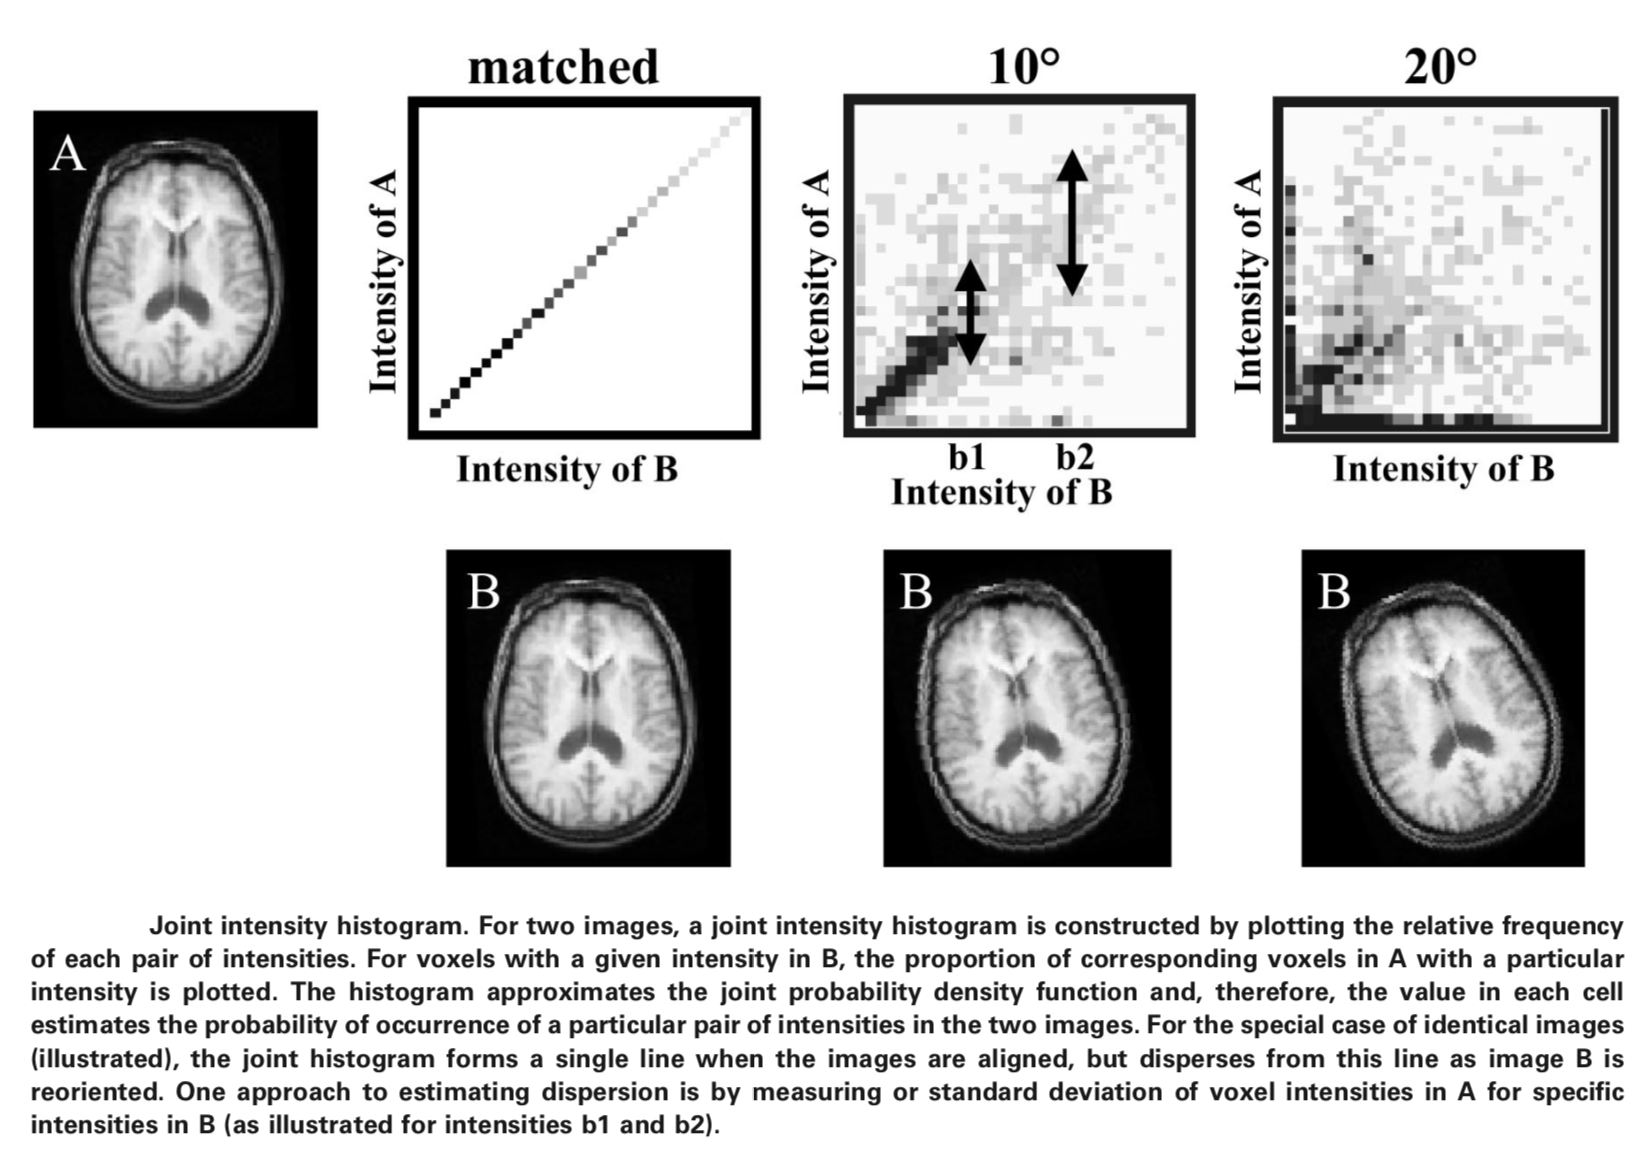
\includegraphics[scale=.5]{figures/hutton_mi.png}
  \caption{\csentence{\cite{hutton_software_2003}} A joint intensity histogram, otherwise known as MI.}
  \label{fig:hutton_mi}
\end{figure}

\section*{Conclusions}
The future of CAD seems to be pointed in the direction of larger atlas-databases that store high-quality annotated CT and MRI scans \cite{van_ginneken_computer-aided_2011}. Other applications of CAD segmentation and registration methods include multi-modal image fusion--where anatomical images from CT or MRI are combined with functional images from fMRI--and guided and targeted therapy \cite{oliveira_medical_2014}, \cite{hutton_software_2003}. The feasibility of CAD has only strengthened with the parallel-computing power afforded by GPUs, with altasing and active contouring being highly suitable to be implemented on this processor architecture \cite{smistad_medical_2015}. CAD techniques have two main strengths; it can reduce radiation dosage and improve image quality. With image quality, iterative reconstruction methods have been found to improve objective image quality (e.g., streak artefact reduction), although the iterative reconstructed images were subjectively observed to be blotchier \cite{liu_model-based_2014}, \cite{geyer_state_2015}. Clinicians would need to be trained to adjust for the different image appearance.
\par While there are numerous benefits of the CAD techniques that have been discussed, that is not say there are no issues. Cost of such systems can be prohibitive for clinical integration. The design of CAD systems also could be cumbersome to use in daily practice. Then there are concerns about the usefulness. One deficiency with the lesion detection methods used in CT is that their sensitivity, or false positive rate, is below the sensitivity level of a  radiologist. However, there is one benefit to false positive detection; the algorithm flags abnormalities that were missed. Regardless, this requires a human (clinician) to ignore the false positives. The concern of the accuracy of such CAD methods are also centred on the potential for reduced specificity (false negatives). The data do not support these concerns. False positives have been positively correlated to true positive detection \cite{van_ginneken_computer-aided_2011}. These concerns also do not consider the another facet of diagnosis: quantification. In a sense, we can redefine the problem trying to be answered with CAD. Instead of flag regions of concern, these CAD system can report meaningful scores or metrics. This means that feature extraction and classification are absent from such a system. For example, instead of flagging a region as a tumour, the CAD system would be able to track the growth rate and size of a tumour. According to \cite{van_ginneken_computer-aided_2011}, radiologists report that quantification takes a larger share of their time in the day, not detection. These `bugs' all become moot as the methods, now afforded more computing-power with GPUs, become more accurate and robust. The maximisation and minimisation approaches (e.g., using the Lagrangian), while a challenge on traditional CPUs, are more efficient on GPUs.
\par To conclude, I hope that this primer, which I acknowledge is hardly comprehensive, has illuminated the state-of-the-art of clinical CAD. As is the case with many engineering challenges like CAD, the theory does not always satisfy the practical constraints. Integrating computer vision and machine learning into medicine is no exception. While algorithms may be powerful and rigorous, implementing them \textit{in silico} is another question. Real hardware constraints in forms of time, cost, and energy limit the algorithms that can be implemented and their applications. For decades, CPUs had been a roadblock. The costs could simply not justify wide-spread use of CAD. While the implementation of GPUs may have changed that, they have not been a panacea. Some CAD algorithms are not efficient, accurate, or robust enough to justify. Further research to improve the algorithms and hardware will need to continue. I am aware of one area of research that seeks to design processor hardware for the purpose of solving the highly parallel computations used in machine learning. (One of the leading researchers in this field is UW Electrical Engineering professor C. J. Richard Shi.) GPUs, while conducive for parallel processing, were not designed and tailored with machine learning and computer vision in mind. This hardware design approach will only benefit CAD such that it could become commercially and clinically viable.

%%%%%%%%%%%%%%%%%%%%%%%%%%%%%%%%%%%%%%%%%%%%%%
%%                                          %%
%% Backmatter begins here                   %%
%%                                          %%
%%%%%%%%%%%%%%%%%%%%%%%%%%%%%%%%%%%%%%%%%%%%%%

% \begin{backmatter}

% \section*{Competing interests}

% \section*{Author's contributions}

% \section*{Acknowledgements}

%%%%%%%%%%%%%%%%%%%%%%%%%%%%%%%%%%%%%%%%%%%%%%%%%%%%%%%%%%%%%
%%                  The Bibliography                       %%
%%                                                         %%
%%  Bmc_mathpys.bst  will be used to                       %%
%%  create a .BBL file for submission.                     %%
%%  After submission of the .TEX file,                     %%
%%  you will be prompted to submit your .BBL file.         %%
%%                                                         %%
%%                                                         %%
%%  Note that the displayed Bibliography will not          %%
%%  necessarily be rendered by Latex exactly as specified  %%
%%  in the online Instructions for Authors.                %%
%%                                                         %%
%%%%%%%%%%%%%%%%%%%%%%%%%%%%%%%%%%%%%%%%%%%%%%%%%%%%%%%%%%%%%

% if your bibliography is in bibtex format, use those commands:
\section*{References}
\printbibliography[heading=none]


%%%%%%%%%%%%%%%%%%%%%%%%%%%%%%%%%%%
%%                               %%
%% Figures                       %%
%%                               %%
%% NB: this is for captions and  %%
%% Titles. All graphics must be  %%
%% submitted separately and NOT  %%
%% included in the Tex document  %%
%%                               %%
%%%%%%%%%%%%%%%%%%%%%%%%%%%%%%%%%%%

%%
%% Do not use \listoffigures as most will included as separate files

%\section*{Figures}
 % \begin{figure}[!ht]
  %\caption{\csentence{Sample figure title.}}
   %   A short description of the figure content
    %  should go here.}
   
   % \fbox{\includegraphics[scale=.8]{Features.pdf}}
    
    %  \end{figure}

%\begin{figure}[h!]
 % \caption{\csentence{Sample figure title.}
  %    Figure legend text.}
   %   \end{figure}

%%%%%%%%%%%%%%%%%%%%%%%%%%%%%%%%%%%
%%                               %%
%% Tables                        %%
%%                               %%
%%%%%%%%%%%%%%%%%%%%%%%%%%%%%%%%%%%

%% Use of \listoftables is discouraged.
%%
%\section*{Tables}
%\begin{table}[h!]
%\caption{Sample table title. This is where the description of the table should go.}
 %     \begin{tabular}{cccc}
  %      \hline
   %        & B1  &B2   & B3\\ \hline
    %    A1 & 0.1 & 0.2 & 0.3\\
     %   A2 & ... & ..  & .\\
      %  A3 & ..  & .   & .\\ \hline
      %\end{tabular}
%\end{table}

%%%%%%%%%%%%%%%%%%%%%%%%%%%%%%%%%%%
%%                               %%
%% Additional Files              %%
%%                               %%
%%%%%%%%%%%%%%%%%%%%%%%%%%%%%%%%%%%

%\section*{Additional Files}
 % \subsection*{Additional file 1 --- Sample additional file title}
  %  Additional file descriptions text (including details of how to
   % view the file, if it is in a non-standard format or the file extension).  This might
%    refer to a multi-page table or a figure.

 % \subsection*{Additional file 2 --- Sample additional file title}
  %  Additional file descriptions text.


% \end{backmatter}
\end{document}
